Figure~\ref{fig:eager_design} illustrates the main components of EAGER (in
blue) and their interactions. Solid arrows represent the interactions that take place
during application deployment-time, before an application has been validated
for deployment. Short-dashed arrows indicate the interactions that take place
during deployment-time, after an application has been successfully validated.
Long-dashed arrows indicate interactions at run-time.

EAGER is invoked whenever a developer attempts to deploy an application, using
the developer tools available on his/her workstation. In some cloud
implementations these tools could be available as an online service accessed
via a web browser. In either case, the application deployment request is
intercepted by EAGER API Deployment Coordinator (ADC), which then performs the 
required governance checks based on the metadata stored in the Metadata Manager.
Metadata manager stores application names, versions, dependencies, API specifications,
user profiles and API keys.
Governance checks are driven by a set of administrator-specified policies that
are stored along with the ADC. These policy files are written in Python, and make use of 
the following assertion functions:

\begin{figure}
\centering
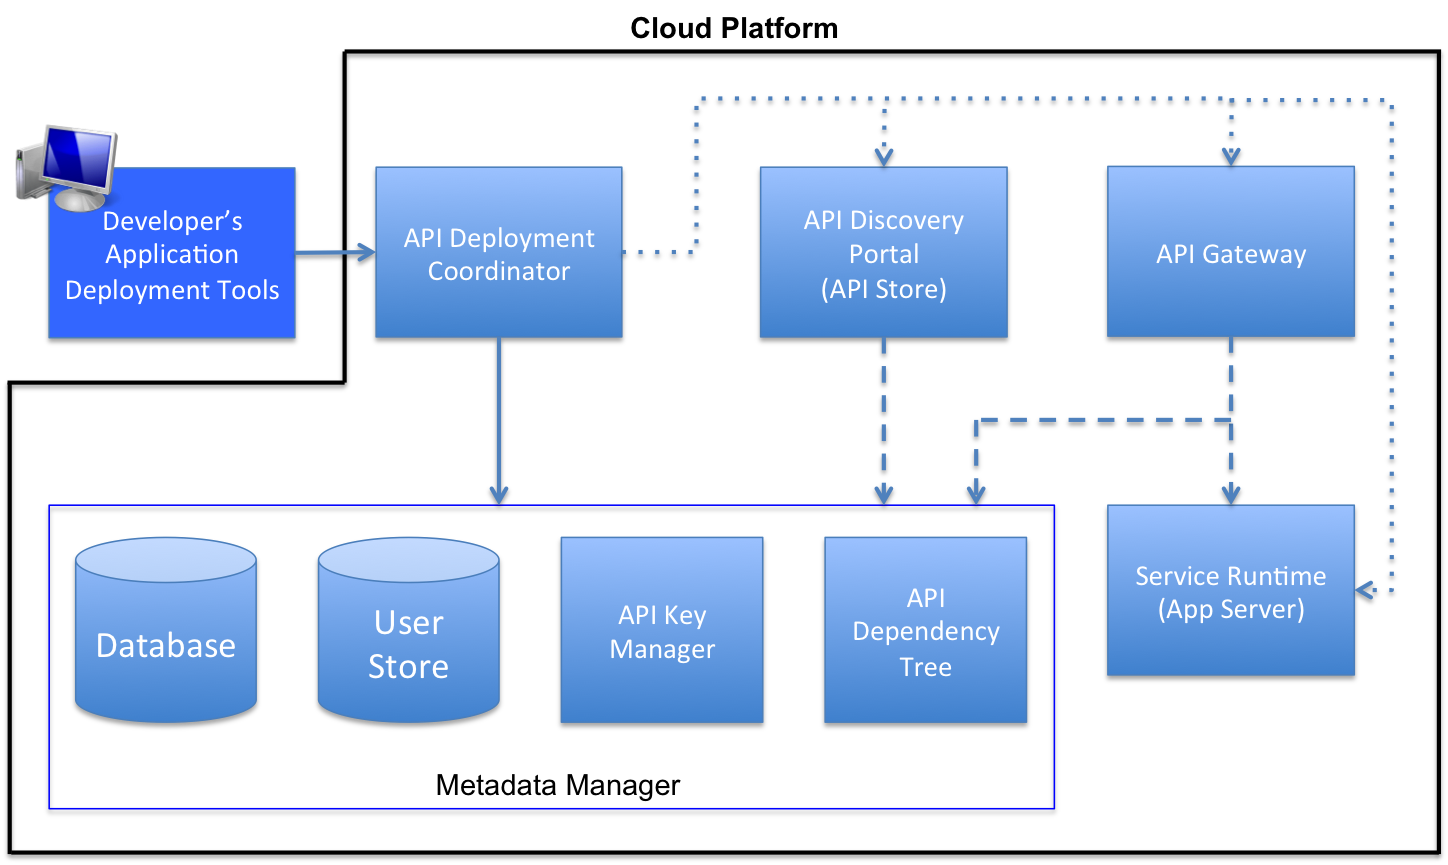
\includegraphics[scale=0.3]{eager_design}
\caption{EAGER Architecture}
\label{fig:eager_design}
\end{figure}

{\footnotesize 
\begin{lstlisting}[language=Python, frame=single]
assert_true(condition, optional_error_msg)
assert_false(condition, optional_error_msg)
assert_app_dependency(app, d_name, d_version)
assert_not_app_dependency(app, d_name, d_version)
assert_app_dependency_in_range(app, name,\
  lower, upper, exclude_lower, exclude_upper)
\end{lstlisting}
}

If a governance check fails (i.e. assertion failure), EAGER will preempt the 
application deployment, and
return an error. Otherwise it proceeds with the application deployment by
activating the deployment mechanisms on the developer's or administrator's
behalf.

The API Discovery Portal is a web GUI that enables application developers to browse and
discover available APIs, and obtain the necessary API keys. The API Gateway intercepts
API calls at runtime and performs security and rate-limiting checks.